\documentclass[upright, contnum]{umemoria}
\depto{DEPARTAMENTO DE CIENCIAS DE LA COMPUTACIÓN}
\author{FRANCISCO JOSÉ CIFUENTES QUIJADA}
\title{Eliminicación de puntos críticos de falla: el caso de Threshold Cryptography Backend}
\auspicio{NIC Chile Research Labs}
\date{SEPTIEMBRE 2015}
\guia{Javier Bustos Jiménez}
\carrera{MAGÍSTER EN CIENCIAS, MENCIÓN COMPUTACIÓN}
\memoria{TESIS PARA OPTAR AL GRADO DE}
\comision{Alejandro Hevia}{Jocelyn Simmonds}{\ }

\usepackage{lipsum}

\begin{document}

\frontmatter
\maketitle

\begin{abstract}
{\lipsum[1-4]}
\end{abstract}

\begin{dedicatoria} % opcional
Una dedicatoria corta. Por ejemplo, \emph{A los creadores de U-Campus}
\end{dedicatoria}

\begin{thanks} % opcional
\lipsum[1-2]
\end{thanks}
\cleardoublepage

\tableofcontents
\listoftables % opcional
\listoffigures % opcional

\mainmatter

\begin{intro}
Desde sus orígenes, nunca se sospechó el grado de penetración y protagonismo que llegaría a alcanzar Internet. De acuerdo a importantes y periódicos estudios sobre dicha red \cite{report:akamai} la tónica de últimos años se podría caracterizar como: Grandes y sostenidos incrementos tanto en el número de conexiones a Internet como en la velocidad de las mismas. Éste factor de alto crecimiento es seguramente la característica fundamental de la llamada ``Era de la información'' que nos ha repletado de dispositivos demandando constantemente acceso a Internet. Un escenario que postula todo un desafío para la infraestructura --tanto de hardware como de software-- disponible de la red.

\section*{Crecimiento de la red}
El gran crecimiento en la cantidad de sistemas tecnológicos interconectados vía Internet en el mundo en los últimos 30 años es algo que no ha dejado indiferente a nadie\footnote{\url{http://www.internetworldstats.com/emarketing.htm}}. Para entender este fenómeno distintos organismos internacionales se dedican periódicamente a realizar estimaciones de dicha cifra. Un caso muy popular de esta labor es el contador global de conexiones móviles a Internet del \emph{GSMA Intelligence}\footnote{\url{https://gsmaintelligence.com/}} el cual recientemente ha estimado en más de 7 mil millones el número de dispositivos móviles con conexión a la red, superando por primera vez al total de la población mundial\footnote{\url{http://www.cnet.com/news/there-are-now-more-gadgets-on-earth-than-people/}}. Una premisa que coincide con el último informe \emph{The State Of Internet} de la corporación \emph{Akamai} \cite{report:akamai} donde se resume el estudio de las principales variaciones en capacidad de acceso, velocidades de acceso, tipos de ataques, etc. a Internet de que disponen distintos países del mundo. Éste estudio corroboró lo que ya ha sido tendencia en los últimos años: Tanto las velocidades de navegación, como el total de conexiones a Internet han aumentado generalizadamente en todo el planeta (Ver figura \ref{fig:akamai_stats}). Las proyecciones a futuro preservan ésta tendencia apostando a que tanto la cantidad de dispositivos como el número de accesos a Internet deberían seguir subiendo \cite{nota:2020}, ello producto de factores como la reducción de costos de producción y la minimización de la tecnología, además de distintas tendencias generadas a raíz del fenómeno de \emph{globalización} que --en gran medida-- nos ha forzado a participar de una sociedad más interconectada en todo el mundo. Olvidando un poco las interpretaciones o justificaciones para ésta situación, el hecho concreto es que existe una directa proporcionalidad entre el número de dispositivos y los requerimientos de accesos a la red, y hoy ambos están en su apogeo de crecimiento.

\begin{figure}[!h]
	\centering
	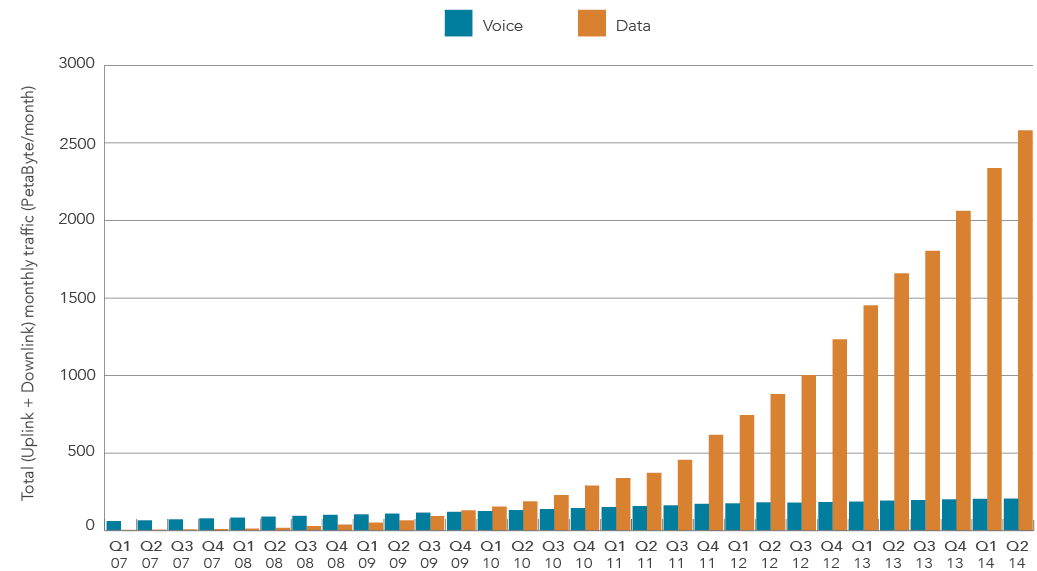
\includegraphics[scale=0.5]{imagenes/conexiones_moviles}
	\caption{Registros de la compañía \emph{Ericsson} ilustrando el crecimiento exponencial en el uso de datos de los dispositivos móviles. Parte del informe de \emph{Akamai} \cite{report:akamai}}
	\label{fig:akamai_stats}
\end{figure}

Más allá del número de dispositivos o la cantidad --o calidad-- del acceso a Internet, las distintas aplicaciones actuales han evolucionado sobre la base de protocolos y sistemas diseñados hace varias décadas, pero exigiendo siempre la mejor performance posible en pos de garantizar buenos tiempos de respuesta. Los protocolos más celebres de la llamada \emph{familia de protocolos de Internet} son TCP e IP. Sin embargo, son decenas los protocolos y mecanismos involucrados en las diferentes fases de comunicación entre computadoras y aplicaciones, que permiten en conjunto la operación de la red de redes como hoy la conocemos.

\section*{El modelo OSI}
La capacidad de conectividad entre 2 distintos dispositivos es resultado del efecto combinado de varias capas de abstracción con responsabilidades divididas. Un diseño de operación que se ilustra en un modelo estándar vigente desde los años 80 es el impulsado por la \emph{Organización Internacional de Normalización} (ISO), mejor conocido como el modelo \textbf{OSI}\footnote{Por sus siglas en inglés \emph{Open System Interconnection}.}. En la práctica, la importancia de éste modelo radica en servir como una referencia técnica que ilustra los límites en las responsabilidades entre componentes que conforman una arquitectura de interconexión de sistemas.

El modelo OSI reconoce 7 capas de abstracción en el proceso de comunicación entre dispositivos (Ver figura \ref{fig:osi7capas}), cada una con obligaciones específicas, pero que combinadas soportan constructivamente un mecanismo de comunicación estándar para sistemas que por él se rijan. El acierto de éste enfoque está en permitir el desarrollo de soluciones modulares y especificas a cada una de las capas, sin interferir entre capas diferentes y manteniendo así la compatibilidad con aplicaciones que ya operen en capas distintas. Las 7 capas en cuestión se describen a continuación:

\begin{figure}[!h]
	\centering
	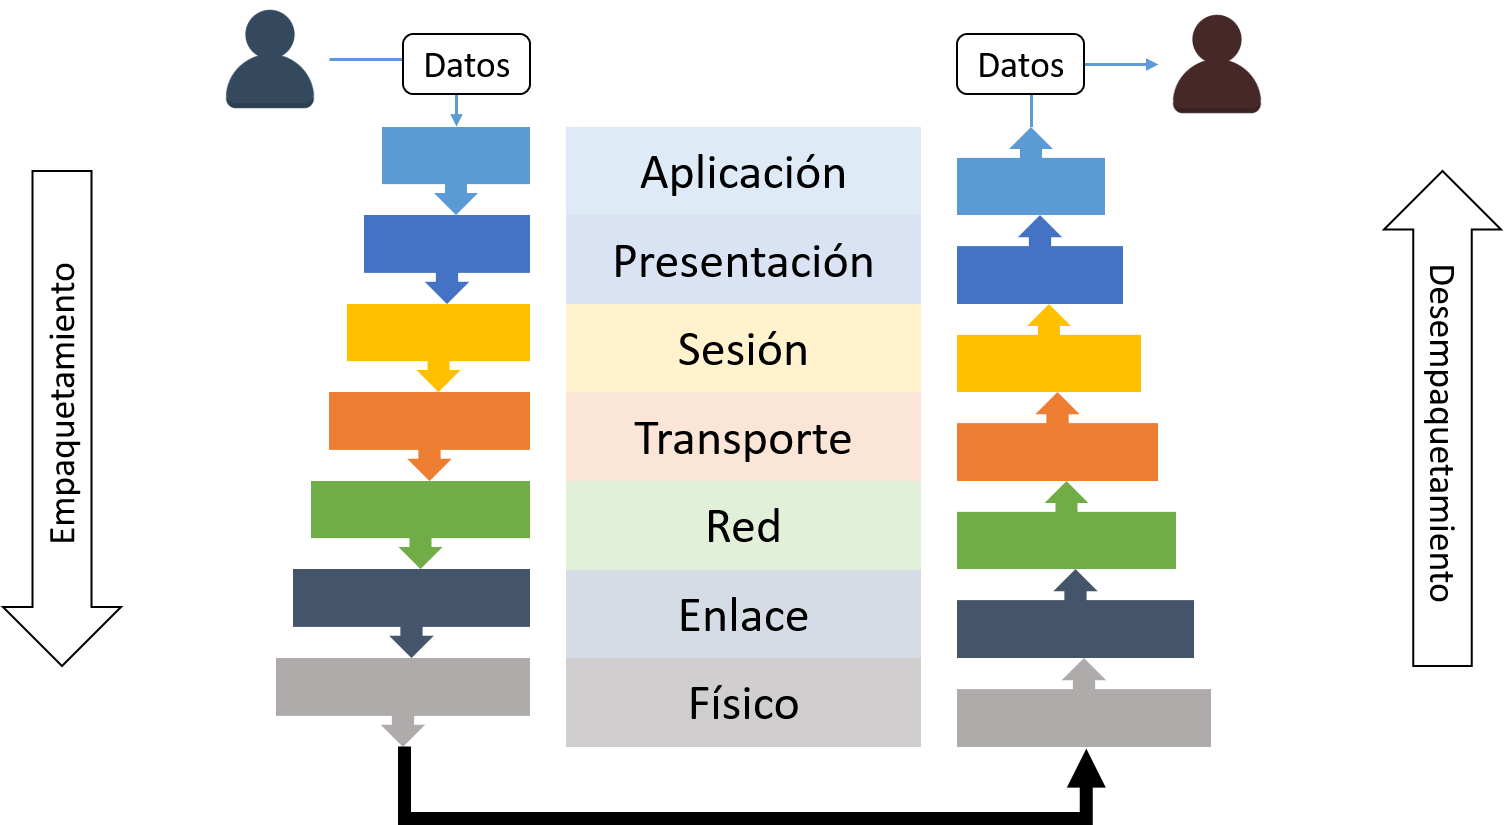
\includegraphics[scale=.45]{imagenes/OSI7Capas.png}
	\caption{Diagrama esquemático de las 7 capas del modelo OSI, ilustrando el proceso de encapsulamiento y desencapsulamiento de datos al ir agregando y removiendo encabezados de capa, según los procesos de empaquetamiento y desempaquetamiento, respectivamente.}
	\label{fig:osi7capas}
\end{figure}

\begin{description}
\item[Capa Física] La capa de nivel inferior en el modelo OSI es la capa física. Es ésta capa la responsible de la topología de la red y de la especificación de los medios materiales que consiguen la transmisión de la información, así como también es responsable de la generación real de la comunicación por medio del envío de la información. Es, en definitiva, la encargada del paso a canales físicos de la información a transmitir.

\item[Capa de Enlace] Es la segunda capa del modelo. Ella se encarga de proveer un mecanismo de direccionamiento físico en una máquina que permita el reconocimiento individual de la misma, proveiendo de un primer identificador a las máquinas en el modelo OSI dado por las direcciones físicas de los dispositivos (\emph{MAC}). Es responsable también de proveer mecanismos de corrección de errores en el proceso de transmisión de datos que pudiesen manifestarse por problemas de la capa física, haciendo dicha comunicación, desde éste punto, confiable.

\item[Capa de Red] Es la tercera capa del modelo OSI. Hace su debut en contextos de multiples equipos interconectados brindando mecanismos de identificación para proveer una capacidad de direccionamiento más amplia con respecto al disponible en las dos primeras capas (que sólo permitian la comunicación entre un par de máquinas, punto a punto). En éste nivel aparece uno de los protocolos más populares en Internet, el denominado protocolo IP que supone un mecanismo de identificación único para cada dispositivo en una red, provisto en base a una dirección homónima. Ésta capa establece la capacidad de ruteo en la comunicación como una responsabilidad de los nodos en una infraestructura en red, haciendo cada componente de la red alcanzable para cualquier otro integrante de la misma.

\item[Capa de Transporte] La cuarta capa del modelo, es la que provee de lleno la capacidad de transporte de datos. En éste nivel se incorporan los también celebres protocolos homónimos: TCP (orientado a la conexión) y UDP (orientado a la mensajería). Ésta capa es también responsible de brindar la capacidad de multiplexación a nivel de una máquina, permitiendo la generación de multiples conexiones desde el mismo dispositivo. Dicho mecanismo lo consigue al incorporar puertos numerados, que sirven como puntos lógicos de comunicación. De ésta manera, a partir de la capa de transporte se establece un paradigma base en el área de redes, en lo que a programación y esquematización de la misma corresponde: La construcción de conexiones \emph{IP:PUERTO}, que son la base del concepto de tuplas de direccionamiento en el proceso de transporte de datos.

\item[Capa de Sesión] Es la quinta capa del modelo OSI. Tal y como su nombre lo indica su función radica en ser la responsible de mantener un control de sesión en una conexión entre extremos, proveiendo mecanismos de corrección y reconexion en caso de interferencia de una operación entre máquinas. Es responsable de mantener el enlace de comunicación construido en base a las capas inferiores en un proceso de comunicación.

\item[Capa de Presentación] El sexto nivel en el modelo OSI es la capa de presentación, cuya responsabilidad comprende proveer el soporte para dar una correcta interpretación de los datos transmitidos, de manera de conseguir que los datos lleguen de manera reconocible al host de destino. A diferencia de las capas inferiores que se enfocan en los mecanismos de envío de la infromación, ésta capa guarda directa relación con la información transmitida y con su correcta interpretación final.

\item[Capa de Aplicación] Es la última -y de más alto nivel- capa de abstracción del modelo OSI. Es la responsible de proveer una interfaz simple a aplicaciones al acceso a mecanismos de comunicación en red. En otras palabras, es la responsible de proveer el servicio de comunicaciones a las distintas aplicaciones que tengan distintos requerimientos de comunicación.

\end{description}

A pesar de que el modelo OSI plantea responsabilidades delimitadas a cada capa de abstracción, la correspondencia de dicho estándar teórico en la práctica es una labor que queda supeditada a los programadores de sistemas operativos. Finalmente son ellos los que, en mayor o menor medida, hacen corresponder para con el modelo las implementaciones finales de los módulos de red de un sistema.


\section*{Familia de Protocolos de Internet}
El conjunto de múltiples protocolos que facultan a los sistemas con mecanismos de interconexión comprende a varios cientos que se distribuyen entre las distintas capas del modelo OSI. A este conjunto se le denomina \emph{Familia de Protocolos de Internet}. Sin embargo, históricamente se le ha prestado especial atención a un subconjunto de ellos que son estructurales en la infraestructura predominante de Internet y que rigen la misma, hablamos del conjunto de protocolos \textbf{TCP/IP}.

La arquitectura de los protocolos TCP/IP sigue la inspiración del modelo OSI en las responsabilidades a soportar --a pesar de romper la estructura de capas del mismo-- combinando algunas responsabilidades de dicho modelo en funciones únicas y obviando otras. Un ejemplo de esto se puede apreciar en la tabla \ref{tabla:tcpiposi} que ilustra la correspondencia de los protocolos del conjunto TCP/IP con su atribución según el modelo OSI.

\begin{table}[h!]
\centering
\begin{tabular}{|c|p{4cm}|l|p{5cm}|}
\hline
\multicolumn{1}{|c|}{\textbf{\begin{tabular}[c]{@{}c@{}}Ref. OSI\\ Nº de capa\end{tabular}}} & \multicolumn{1}{c|}{\textbf{\begin{tabular}[c]{@{}c@{}}Equivalente \\ de capa OSI\end{tabular}}} & \multicolumn{1}{c|}{\textbf{Capa TCP/IP}} & \multicolumn{1}{c|}{\textbf{\begin{tabular}[c]{@{}c@{}}Ejemplos de\\ protocolos TCP/IP\end{tabular}}} \\ \hline
5,6,7                                                                                        & Aplicación, Sesión, Presentación                                                                 & Aplicación                                & NFS, NIS, DNS, LDAP, telnet, ftp, rlogin, rsh, rcp, RIP, RDISC, SNMP y otros.                         \\ \hline
4                                                                                            & Transporte                                                                                       & Transporte                                & TCP, UDP, SCTP                                                                                        \\ \hline
3                                                                                            & Red                                                                                              & Internet                                  & IPv4, IPv6, ARP, ICMP                                                                                 \\ \hline
2                                                                                            & Vínculo de datos                                                                                 & Vínculo de datos                          & PPP, IEEE 802.2                                                                                       \\ \hline
1                                                                                            & Física                                                                                           & Red física                                & Ethernet (IEEE 802.3), Token Ring, RS-232, FDDI y otros.                                              \\ \hline
\end{tabular}
\caption{Comparativa de correspondencia de algunos protocolos de la familia de Internet de acuerdo al modelo OSI.}
\label{tabla:tcpiposi}
\end{table}
%\url{https://docs.oracle.com/cd/E19957-01/820-2981/6nei0r0r9/index.html}

\subsection*{UDP}
UDP \cite{rfc:768} es un protocolo de la familia de protocolos de Internet con funciones a nivel de la capa de transporte según el modelo OSI, que se caracteriza por ser un protocolo orientado a mensajes, vale decir, por permitir enviar mensajes a través de la red sin necesidad de establecer previamente una conexión con el equipo receptor (situación que si ocurre y es característica de los protocolos orientados a la conexión como es el caso de TCP).
%[OSI reference model—The ISO model of architecture for open systems interconnection]%

Ésta naturaleza de UDP tiene varias implicancias:
\begin{itemize}
\item En primer lugar, ser un protocolo orientado a mensajes supone una premura en el envío de información, ello significa que éste protocolo no verifica la correctitud en la recepción de los datos enviados. En ese sentido, UDP es lo que se denomina un protocolo \textbf{no fiable}.
\item Por otro lado, UDP trabaja en estados denominados \textbf{sin conexión}, lo que significa que no hay una verdadera sincronización entre origen y destino. Esto supone el uso de operaciones del tipo asíncronas las que hacen más flexible la comunicación entre los extremos.
\end{itemize}

Por su funcionamiento, la anatomía o estructura de un paquete UDP es bastante simple (Ver fig. \ref{fig:datagramaudp}). Al ser un protocolo orientado al envío de mensajes, los paquetes disponen de pocos campos de información, de manera de evitar sobrecargar los mismos en su transferencia. Así mismo, en éste nivel los paquetes se denominan \emph{datagramas}. Los encabezados de un paquete UDP comprenden: \textbf{Puerto de Origen/Destino}, que hace referencia a los puntos de conexión de la capa Transporte del modelo OSI y \textbf{Longitud del Mensaje} y \textbf{\emph{Checksum}}\footnote{Corresponde a un valor generado a partir de una función matemática que se aplica sobre datos para corroborar la integridad de los mismos y su correcta recepción tras un envío.}, que sirven como componentes de verificación del paquete mismo.

\begin{figure}[!h]
	\centering
	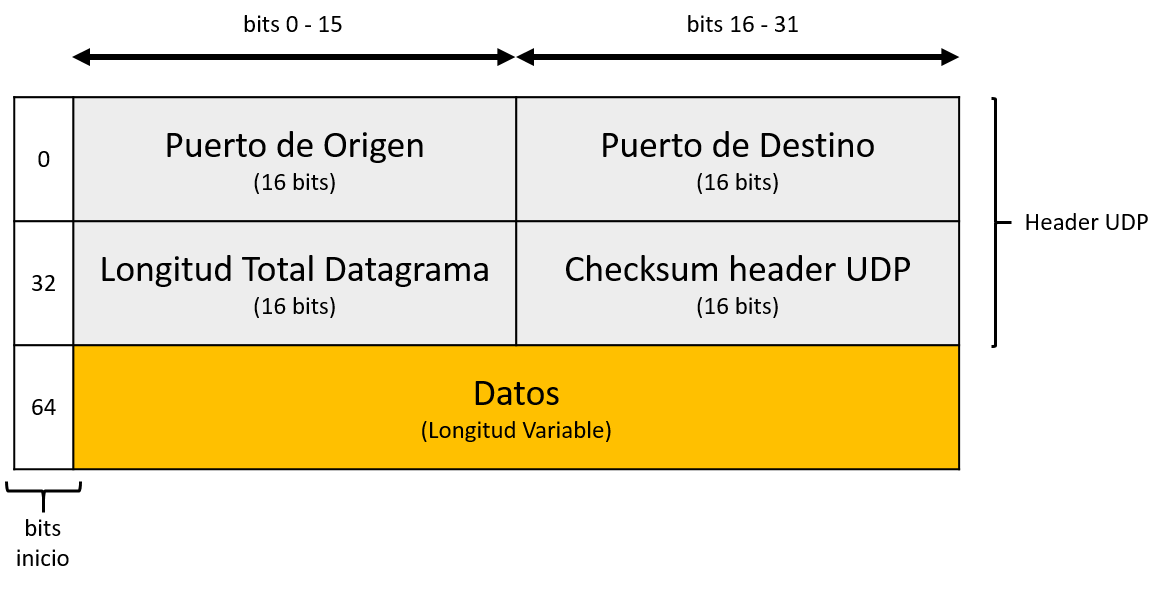
\includegraphics[scale=.55]{imagenes/estructuraUDP.png}
	\caption{Estructura de un paquete UDP con detalle del tamaño de sus encabezados de capa de transporte.}
	\label{fig:datagramaudp}
\end{figure}

El protocolo UDP se estandarizó el año 1980, sin embargo su aplicación ha sido muy variada en distintos sistemas modernos. Hoy por hoy UDP es uno de los componentes estructurales de la Internet estando presente en diversas aplicaciones que van desde transmisiones en uso intensivo de datos para redes de alta velocidad \cite{udp:highbandwidth}, hasta mecanismos de transmisión de video \cite{udp:video}, entre otros. Sin embargo, una de las aplicaciones más importantes (sino la más trascendental) de éste protocolo en la infraestructura de Internet, es su labor en el servicio DNS.

\subsection*{DNS}
\label{section:dns}
Todo dispositivo conectado a una red de computadoras se identifica a si mismo por la denominada \emph{dirección IP}, un identificador que permite referenciarlo y diferenciarlo de otros dispositivos conectados a la misma red, definido por el nivel 3 del modelo OSI. No obstante para poder conectarse con un recurso disponible en Internet, generalmente los dispositivos consultan por lo que llamamos \emph{nombres de dominio}, que son identificadores con carácter semántico para los usuarios que definen una red de identificación asociada a un grupo de dispositivos o equipos conectados a la red \cite{wiki:nombre_dominio}. Éste mecanismo de traducciones se conoce como \textbf{servicio DNS} y es vital para el funcionamiento de Internet como lo conocemos.

El servicio DNS \cite{rfc:1034, rfc:1035} opera como una base de datos distribuida que permite resolver consultas de manera jerarquizada basado en un principio de consultas recursivas. Frente a una consulta por un nombre de dominio, el primer paso es la resolución de la misma empleando datos de la caché local del servicio DNS del sistema (Esto es, emplear información previa en caso de que el nombre consultado ya hubiese sido preguntado anteriormente). En caso de encontrarse la respuesta en la caché local, se responde la consulta con ésta información y el proceso finaliza. En caso de que la consulta no coincida con algún registro local, se promueve el proceso de resolución de nombre al servidor DNS preferido (Configurado en el sistema).  

Frente a una consulta, un servidor DNS hace una verificación en su información local para determinar si tiene autoridad para responder al nombre solicitado en función de la zona que tenga configurada. En caso de que el nombre consultado coincida con algún registro de dicho servidor, el servidor usa ésta información para responder la consulta con autoridad y finaliza el proceso. En caso de que éste servidor no disponga de una entrada con el nombre pedido, se verifica en su caché local en caso de que previamente el servidor hubiese formado parte de una cadena de resolución para el nombre pedido, en cuyo caso puede responder con la resolución almacenada en caché y finalizar la consulta. Si tras todas las verificaciones anteriores (Sobre los registros de la zona DNS y de caché de resoluciones) el nombre de dominio consultado no registra apariciones en el servidor DNS preferido, la consulta se promueve recursivamente a otros servidores DNS con sugerencias de raíz para el nombre solicitado, de manera de poder conseguir una respuesta autoritativa en cada caso. Para esto la consulta se resuelve desde el dominio de nivel superior, resolviendo desde lo general a lo particular del nombre de dominio. Un ejemplo de resolución del dominio dcc.uchile.cl se ilustra en la imagen \ref{fig:dns}

\begin{figure}[!h]
	\centering
	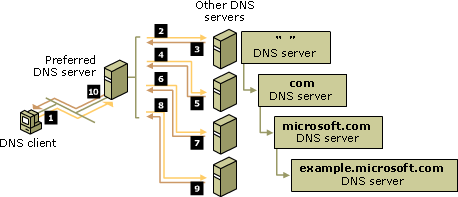
\includegraphics[scale=0.75]{imagenes/dns-system.png}
	\caption{Diagrama de operación del servicio DNS ilustrando comunicación entre servidores de dicho tipo.}
	\label{fig:dns}
\end{figure}

En la práctica, el servicio DNS emplea el protocolo UDP para la comunicación desde y hacia los servidores de dicho tipo, esto pues las características de una consulta DNS contemplan:

\begin{itemize}
\item \textbf{Consultas Auto-Contenidas} La información de una consulta DNS calza fácilmente en un paquete de UDP.
\item \textbf{Orden Irrelevante} Los requerimientos DNS no necesitan ser procesados en un orden establecido. Sin embargo, si requieren ser eventualmente procesados y ello en el menor tiempo posible. Un factor que justifica el uso de UDP al ser precisamente un protocolo orientado a mensajes.
\end{itemize}

De esta manera, las características anteriores justifican el uso de UDP como protocolo para la comunicación entre los servidores DNS.

El escenario antes descrito explica el por qué UDP tiene una participación de gran importancia en las redes actuales (en especial sobre Internet) y además, dado el sostenido aumento en el número de conexiones explicado en las secciones previas, da cuenta de cómo el tráfico de éste tipo de comunicación representa una porción muy significativa en la operación de las redes modernas. Una situación que con el paso de los años ha exigido cada vez mejores técnicas de procesamiento para dar mejores tiempos de respuesta.

\section*{Planteamineto de Investigación}

La pregunta natural entonces es: ¿Están capacitados los servidores DNS para responder tal cantidad de peticiones correctamente? Más allá de la respuesta a ésta interrogante el hecho es que, para su correcta operación, los servidores DNS deben garantizar bajos tiempos de respuesta y eficiencia en su operación en todo escenario.

Un excelente enfoque para abordar la problemática anterior mora en usar paralelismo, ósea, aprovechar la independencia entre peticiones DNS para procesar varios requerimientos a la vez de manera simultánea. En la práctica, dicha solución propone compartir una misma interfaz de conexión (denominada \emph{Socket}) entre varios hilos de ejecución. Ésta práctica supone --en teoría-- un incremento en el rendimiento de operación del procesamiento de las peticiones DNS, siempre que existan procesadores disponibles para atender cada hilo de forma independiente.

Sin embargo, los resultados al evaluar el enfoque antes propuesto revelan un preocupante e insospechado panorama donde el rendimiento de los servidores DNS no escala al incorporar directamente paralelismo en el procesamiento de peticiones como se esperaría \cite{tesis:diegoDCC}. Éste fenómeno ha sido repasado por distintos grupos de investigación en el área como Facebook, Toshiba \cite{post:facebook, paper:toshiba} e incluso industrias nacionales como NIC Chile, pero sin mayor solución más que delegar dicha responsabilidad a unidades estructurales del sistema operativo (como el kernel del sistema operativo) de donde tampoco se han conseguido mayores mejoras.

La pregunta entonces es ¿Por qué el sistema de procesamiento de peticiones DNS no escala al incorporar paralelismo directamente? Una sospecha interesante propone que probablemente el sistema de procesamiento de paquetes para UDP (que es el protocolo involucrado en las peticiones DNS) podría tener imperfecciones a nivel de diseño en el sistema operativo que no garantizarían su óptimo funcionamiento en condiciones de concurrencia, sugiriendo como responsable del problema a un defecto de contención a nivel de estructuras compartidas del sistema operativo. Sin embargo, dicha hipótesis no ha sido comprobada ni desmentida. Por otra parte, determinar la causa del problema anterior significa un tremendo desafío pues implica trabajar a nivel del núcleo del sistema operativo, que combina diversos paradigmas y enfoques de programación incorporados a lo largo de su desarrollo, unido a la dificultad inherente de trabajar analizando un sistema complejo como lo es el kernel mismo.

El presente trabajo plantea precisamente un estudio amplio que reune las principales sospechas de investigación vigentes del problema al momento de su desarrollo, de manera de identificar y analizar las distintas componentes responsables del problema detectado, así como también el estudio de alternativas para palear dicha situación.


\end{intro}
\chapter{Primero}
\lipsum[1-3]
\begin{defn}[ver \cite{KAR00}] Definición definitiva $$\frac{d}{dx}\int_a^xf(y)dy=f(x).$$\end{defn}
\chapter{Segundo}
\lipsum[50-60]
\begin{conclusion}

Como se expuso en el presente trabajo, el inminente crecimiento de las redes de computadoras y el explosivo aumento en el uso de distintos dispositivos que demandan conectividad, hacen que volver la Internet más robusta, disponible y más eficiente sea una prioridad. Entendiendo como parte crucial de dicha labor el trabajo del servicio DNS, postular mejoras que optimicen su operación es un ejercicio plenamente justificado en pos de brindar una mejor performance sobre la red.

A través del \textbf{estudio de llamadas a sistema} se pudo

Con respecto al \textbf{estudio de canales de comunicacion de hardware}, centrado en la dinámica de los performance counters disponibles en el sistema, se

Por otro lado, nuestro \textbf{estudio de distribución de carga} usando processor affinity dio

De esta forma, se pudo corroborar responsabilidades transversales y cruzadas entre las sospechas vigentes del problema estudiado. Trasnversales pues todas las sospechas resultaron ser corroboradas experimentalmente, dando a entender que --En mayor o menor grado-- el diseño de operación de las interfaces de red de Linux no incorpora en su diseño una aplicación que admita concurrencia en el consumo de información, limitando así la capacidad de optimizaciones usando la estratégia de paralelísmo a secas. Y Cruzadas, en el sentido de que los factores responsables de cada sospecha resultan repetirse entre cada caso --siendo principal actor en este sentido el spinlock de protección de la estructura socket--.

Resulta interesante que al día de hoy, el problema estudiado sigue vigente y abierto a nuevas propuestas de soluciones. En esta misma línea, recientemente Facebook, a través de su equipo de desarrollo de kernel ha postulado modificaciones al núcleo de Linux que permitan hacer un uso más flexible en el consumo concurrente de datos desde estructuras protegidas por medio de estructuras denominadas \emph{Blk-mq} \cite{post:facebookFin}, que van en busca de aprovechar consumo distribuidos de colas usando lecturas exclusivas por cada CPU. Un enfoque que aprovecharía de mejor manera las interacciones de hardware del sistema al tener accesos más localizados que lo detectado en nuestro estudio de \emph{Performance Counters} e inspirado sobre la misma idea que nuestro estudio de \emph{Processor Affinity} pero implementado directamente a nivel del kernel. Por otro lado, recientes publicaciones de XXXX muestran como aprovechar arquitecturas NUMA a modo de incrementar el rendimiento de operaciones sobre estructuras compartidas, nuevamente, un enfoque similar al que se repasó en nuestra investigación por medio de \emph{Processor Affinity}.

Finalmente, se postuló una solución basada en un módulo del kernel para Linux que, bajo un escenario de operación fiel al caso de estudio presentado, se presenta plenamente comparable con reuseport --La mejor opción disponible para palear el problema estudiado en cuestión--, y siendo a su vez competitivo en rendimiento con este último, brindando en la práctica un desempeño que es muy similar. Por otro lado, la solución desarrollada cuenta con una característica de balanceo de trabajo que ni el mismo reuseport incorpora, la que brinda una distribución de tiempos de trabajo más equitativa entre los sockets que trabajan conjuntamente, con respecto a reuseport. Por otro lado, el producto final es una solución extensible, modular y modificable, lo que garantiza su fácil adaptación para escenarios de operación especificos e incluso la capacidad de portar la misma a otras plataformas.

\end{conclusion}

% \input{glosario.tex} % opcional

\bibliographystyle{plain}
\bibliography{bibliografia}

% \input{anexo_apendices.tex} % opcionales

\end{document}

%%% Local Variables:
%%% mode: latex
%%% TeX-master: t
%%% End:
